\documentclass[12pt]{phage3slides} %

\title[JBrowse and Circos Update]{JBrowse and Circos Update}
\author[ER, SH]{Eric Rasche \& Saskia Hiltemann}
%\date{2017-06-29T13:50:00Z}

\begin{document}
\frame{\titlepage}


\section{JBrowse}
{
  \usebackgroundtemplate{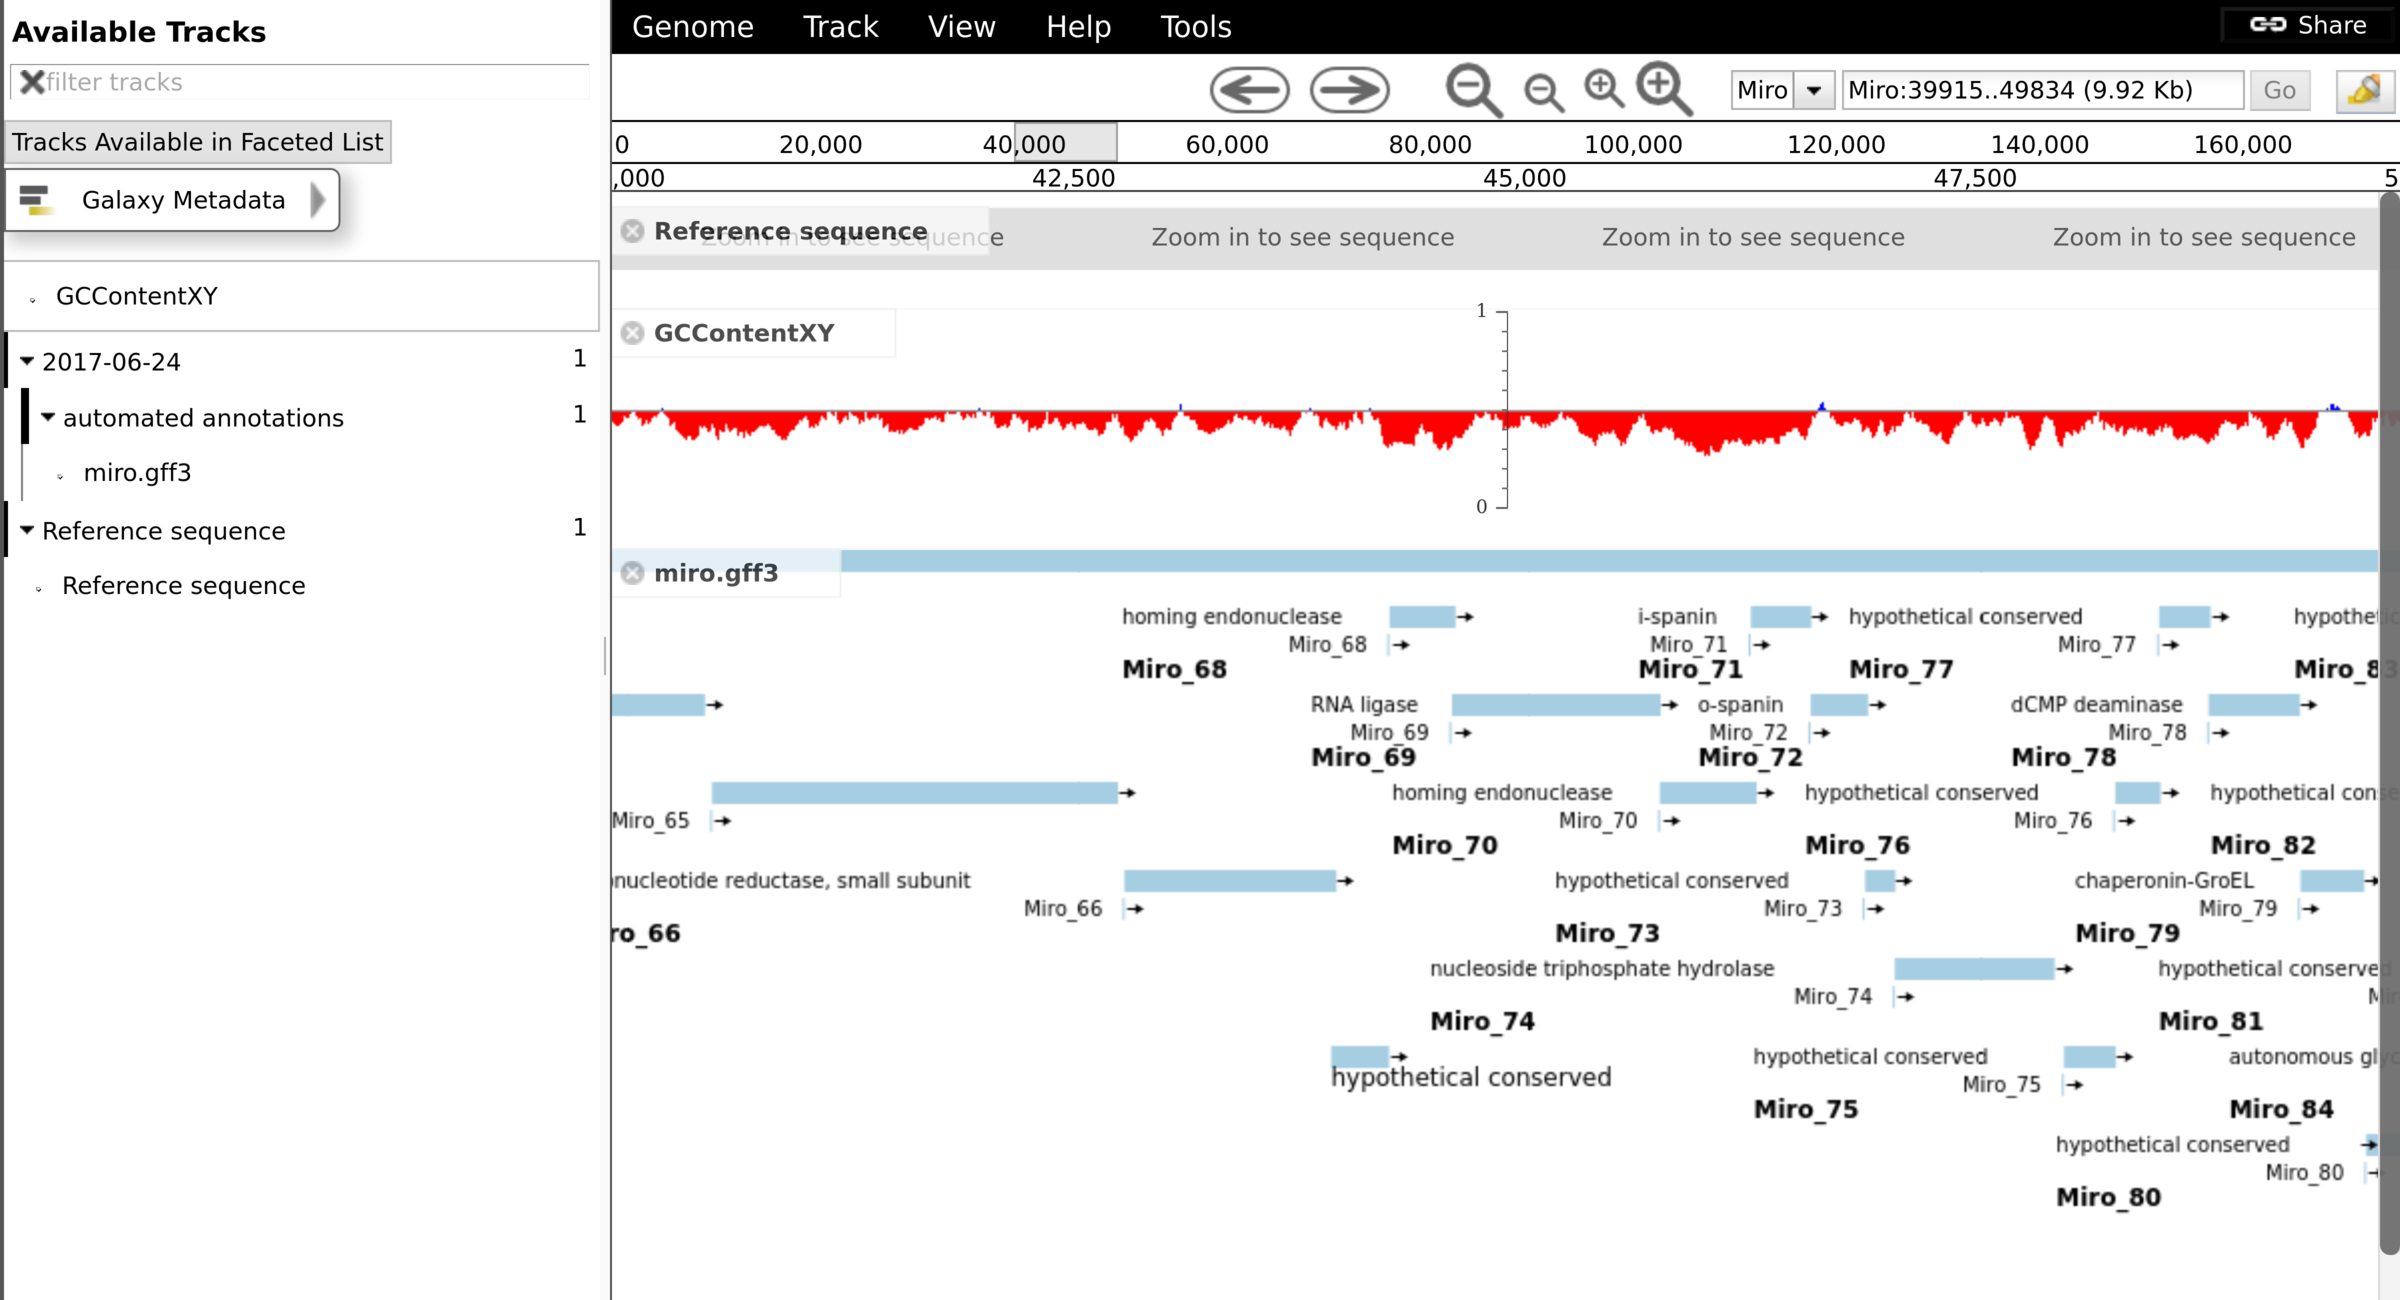
\includegraphics[height=\paperheight]{jbrowse.png}}
  \setbeamertemplate{navigation symbols}{}
  \begin{frame}[plain]
  \end{frame}
}

\subsection{Plugins}
{\setbeamertemplate{navigation symbols}{}
\begin{frame}{JBrowse}
	JBrowse Plugin Support! ({\color{gray}GCContent, ComboTrackSelector, Bookmarks})
	
\includegraphics[width=\textwidth]{plugin-gc.png} \\
	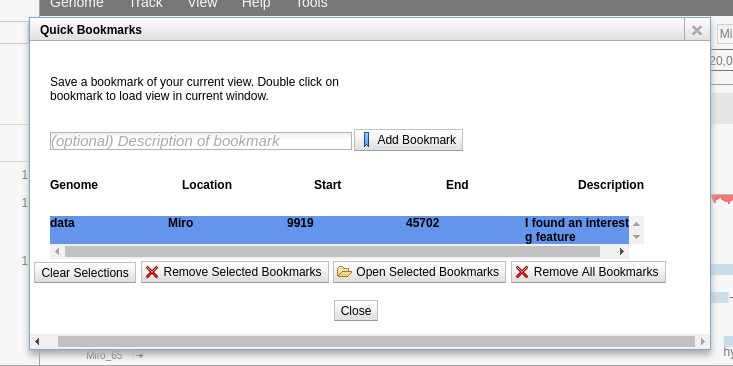
\includegraphics[width=\textwidth]{plugin-book.png}
\end{frame}
}

\subsection{Metadata}
{\setbeamertemplate{navigation symbols}{}
\begin{frame}{ComboTrackSelector}
	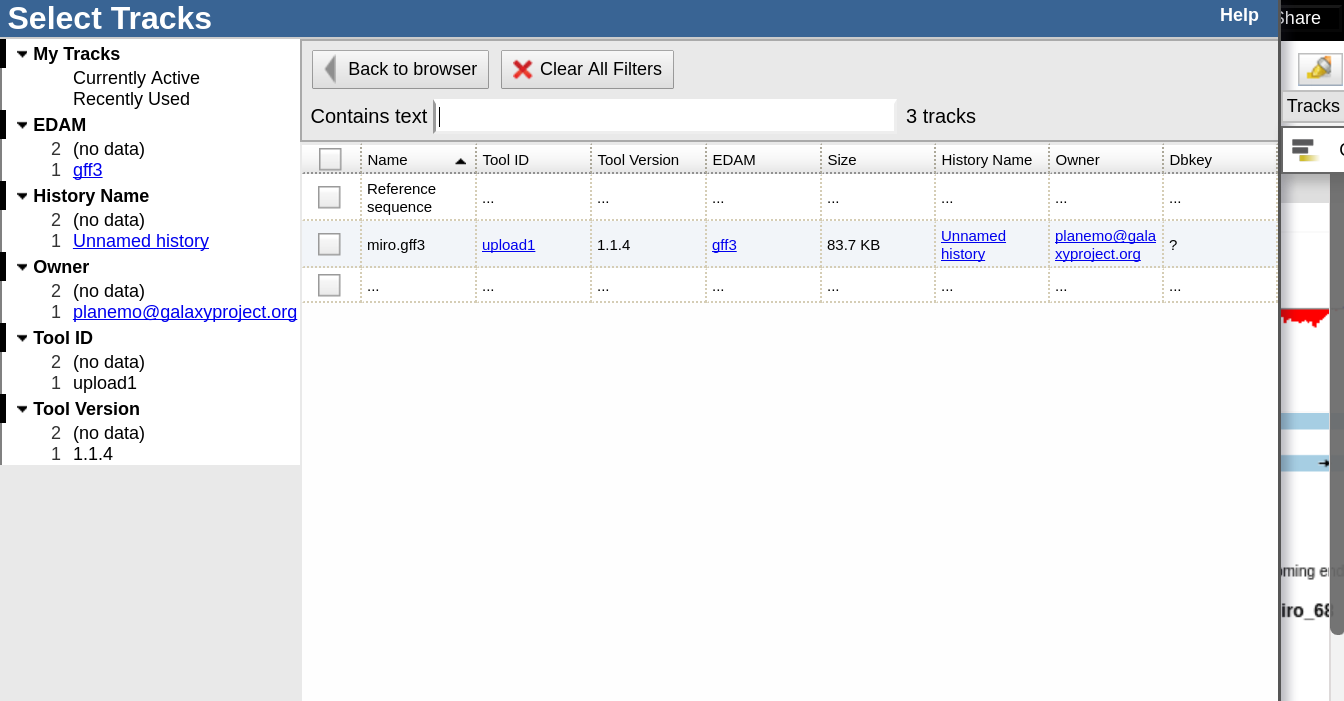
\includegraphics[width=\textwidth]{plugin-combo}
\end{frame}
}

\subsection{Themes}
{
  \usebackgroundtemplate{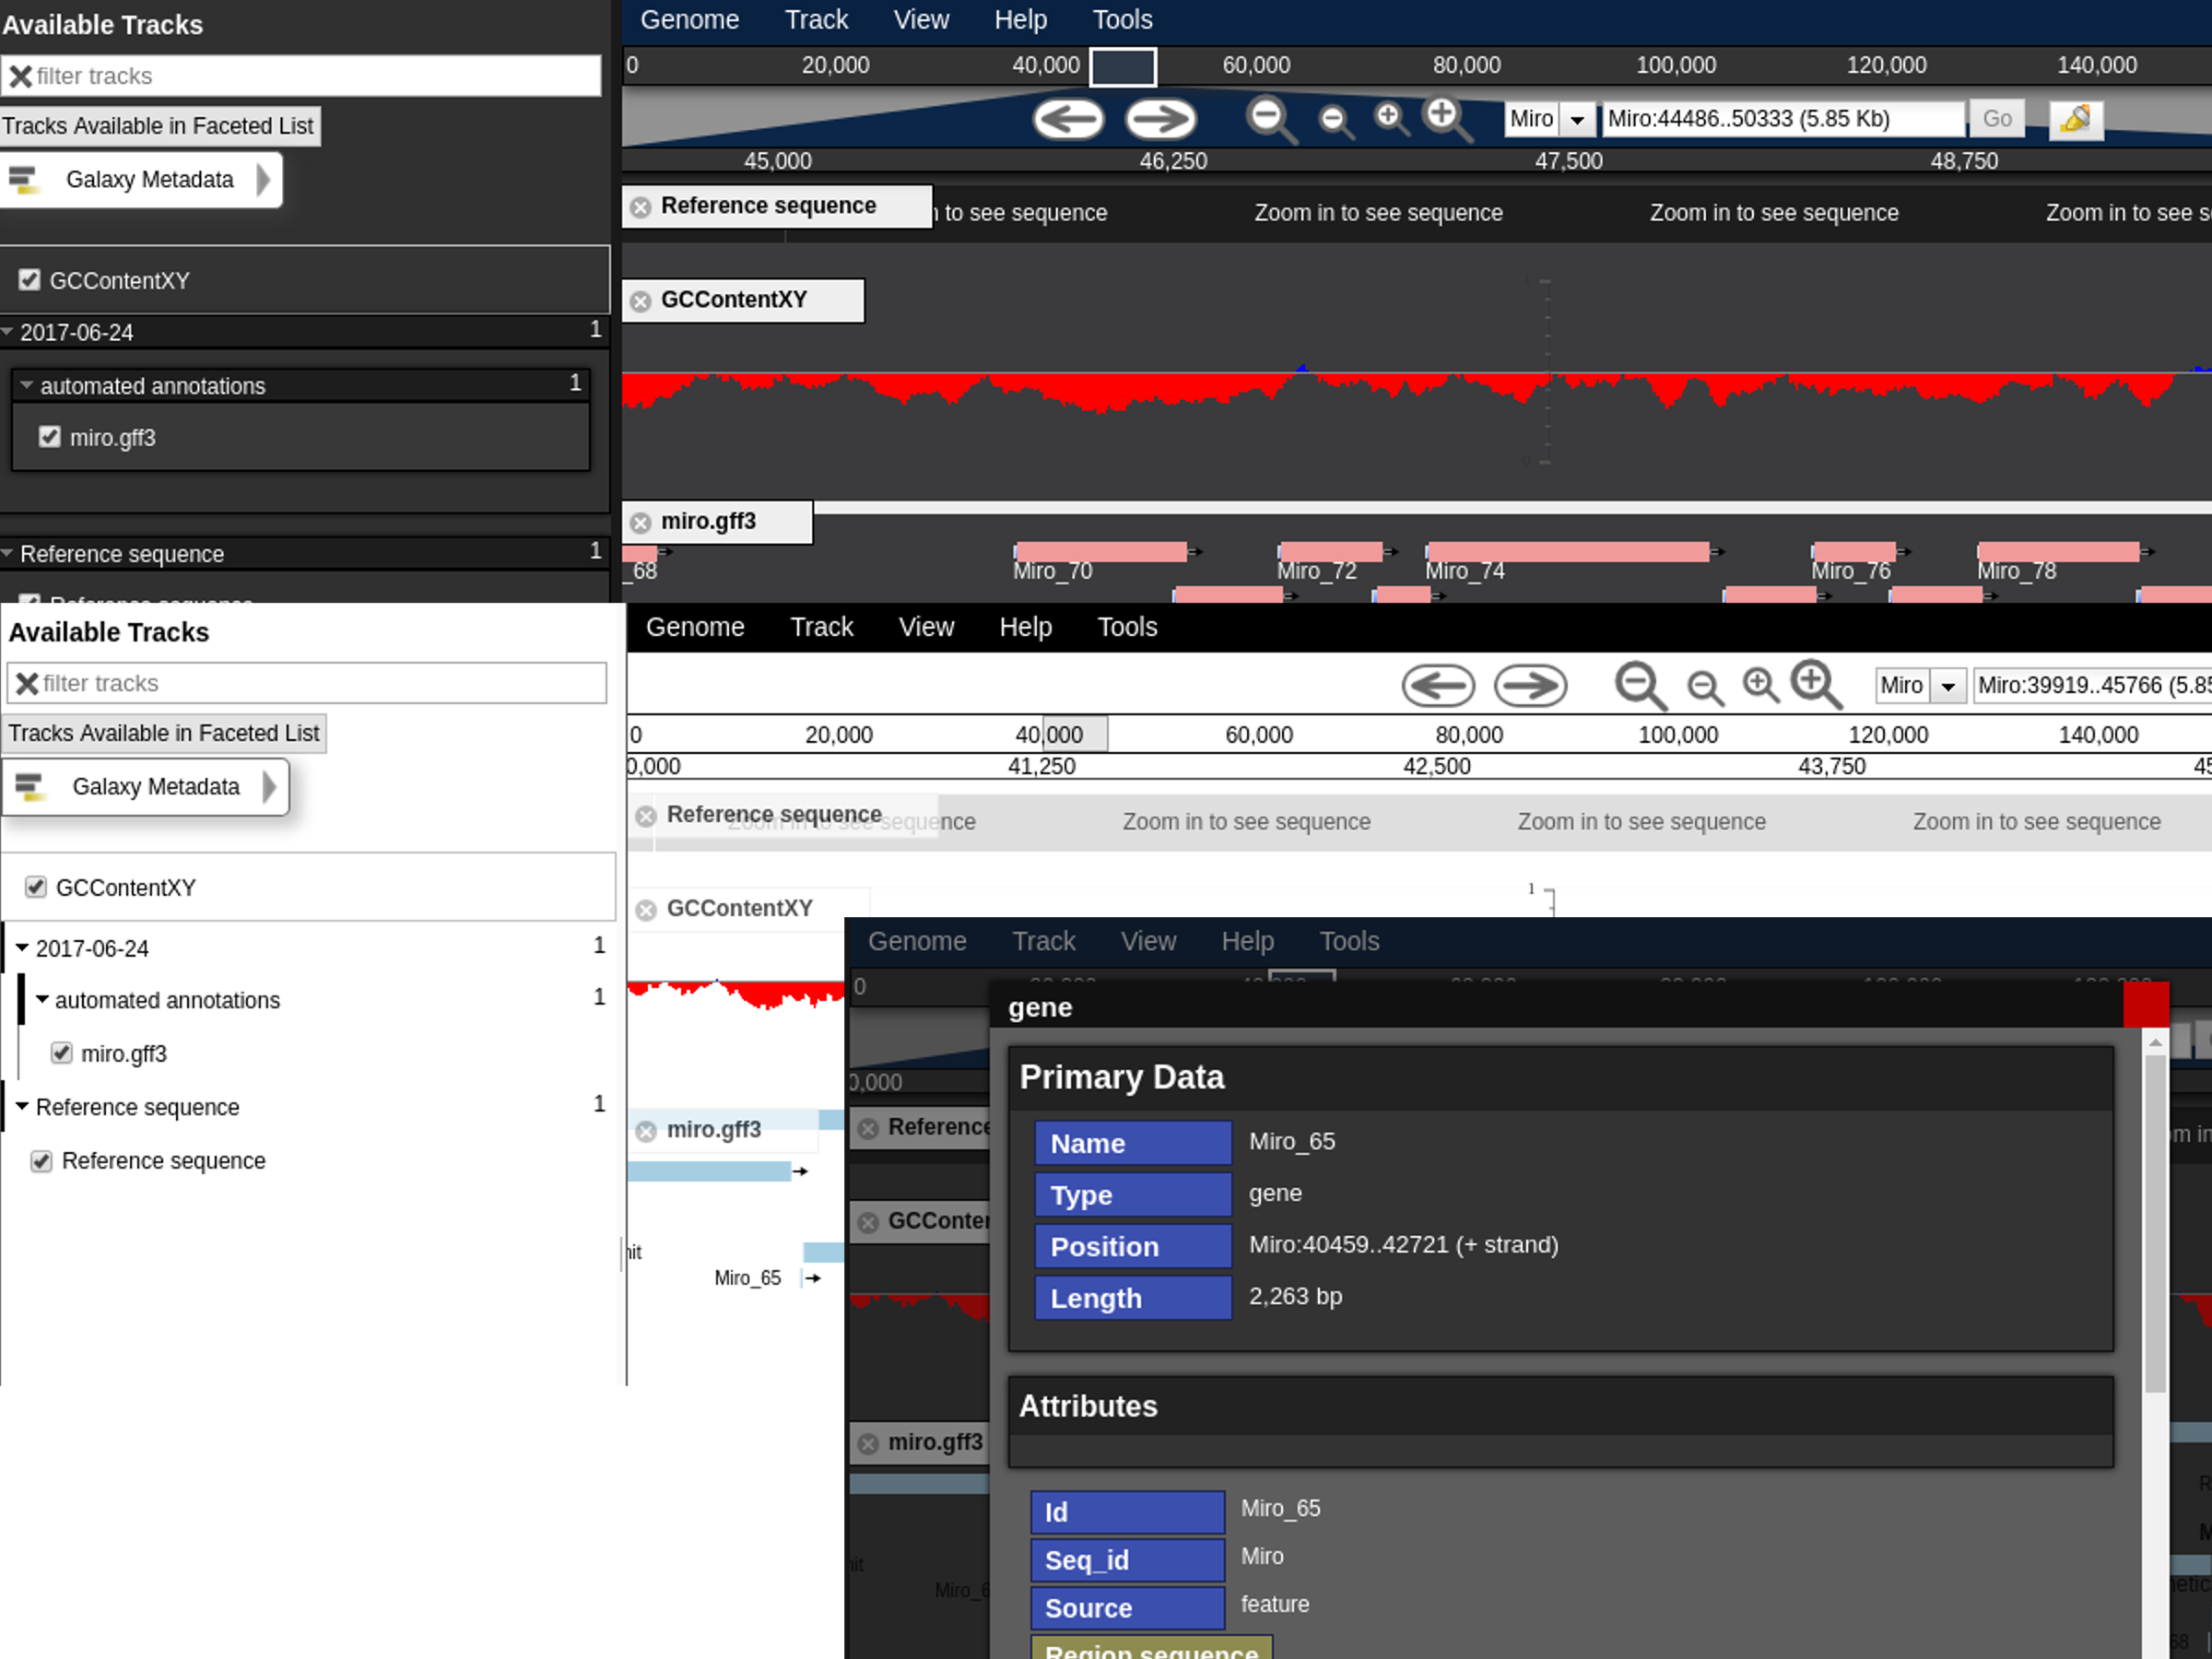
\includegraphics[height=\paperheight]{themes.png}}
  \setbeamertemplate{navigation symbols}{}
  \begin{frame}[plain]
  \end{frame}
}



\section{Circos}
\begin{frame}{Circos}
	\begin{itemize}
		\item Link support
		\item Now mostly feature-complete, support for all major circos features
		\item Soon in IUC
	\end{itemize}
\end{frame}



\section{Q\&A}
\begin{frame}{Q\&A}
	Thank you \\\ \\
	\begin{center}
		\begin{tabular}{rl}
			\end{tabular}\\[1cm]
			%\logosTamuCPT
			\fundingNSFABIannotation
	\end{center}
\end{frame}

\end{document}
